\documentclass[tikz,border=5pt]{standalone}
\usepackage{amsmath}
\begin{document}
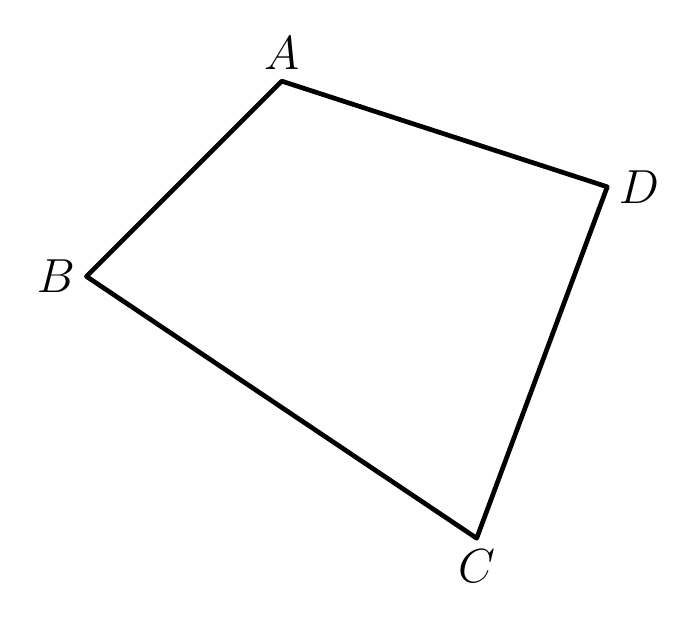
\begin{tikzpicture}[line join=round, line width=1.7pt]
  % Vertices (scale s = 0.021108 cm/px, centred on ink bbox)
  \coordinate (A) at (-0.834,2.923);
  \coordinate (B) at (-3.314,0.443);
  \coordinate (C) at (1.642,-2.882);
  \coordinate (D) at (3.300,1.581);

  % Quadrilateral edges (solid, no diagonals)
  \draw (A) -- (B) -- (C) -- (D) -- cycle;

  % Labels
  \node[above] at (A) {\fontsize{17}{20.4}\selectfont $A$};
  \node[left]  at (B) {\fontsize{17}{20.4}\selectfont $B$};
  \node[below] at (C) {\fontsize{17}{20.4}\selectfont $C$};
  \node[right] at (D) {\fontsize{17}{20.4}\selectfont $D$};
\end{tikzpicture}
\end{document}